\documentclass[dvipdfmx,a4paper,10pt,twocolumn]{jsarticle}

% 余白
\usepackage[top=13mm,bottom=13mm,left=12mm,right=12mm]{geometry}

% 数式
\usepackage{amsmath,amsfonts}
\usepackage{bm}

% 画像
\usepackage{graphicx}
\graphicspath{
  {results/note/}
  {results/error_generator_rate_nbar/top3_pairwise_generator/interaction_mode_maps/}
}
\usepackage[haranoaji]{pxchfon}

% 表
\usepackage{array}

\setlength{\columnsep}{7mm}
\setlength{\parindent}{1em}
\setlength{\parskip}{0pt}

\begin{document}

\title{\vspace{-2em}
M{\o}lmer--S{\o}rensenゲートの解析
\vspace{-1em}}
\author{平井 希空}
\date{\today}
\maketitle
\vspace{-3em}

\section{Motivation}

平均ゲートinfidelityは性能比較には便利だが，コヒーレントな
較正ずれと確率的な散逸を区別できない．特に
M{\o}lmer--S{\o}rensen（MS）ゲートでは，運動自由度を介して
片方のイオンにノイズが生じるweight-1のエラーと
両方のイオンにノイズが生じるweight-2のエラーが同時に生じる．

そこで，Master Equation（ME）から得た量子チャネルをQPTで再構成し，
理想MSゲートを除いた\textbf{error channel}をeffective generatorへ
分解する．さらに，motional heatingとmotional dephasingを同時に
変化させ，単純加算では説明できない2ノイズによって生じる相関の
Pauli成分を特定する．

\section{Prior work \& Method}

MSゲートは二つの波長の異なるレーザーにより振動モードを介して、
\begin{equation}
 U_{\rm MS}=\exp(i\pi XX/4)
\end{equation}
を実装する\cite{MS}．本計算ではmotional heating，
motional dephasing，spin dephasing，photon scatteringを含む
MEを解き，16個の入力演算子からQPTチャネル
$\mathcal E$を構成する\cite{QPT}．

理想操作を除いたerror channelを
\begin{equation}
 \mathcal E_{\rm err}
 =\mathcal U_{\rm MS}^{\dagger}\circ\mathcal E
 \label{eq:error_channel}
\end{equation}
と定義する．これをCPTPチャネルへ射影し，Pauli transfer matrix
$R_{\rm err}$に変換する．
ここで、1ゲート当たりのeffective generatorを
\begin{equation}
 K=\log R_{\rm err}
\end{equation}
とし，
\begin{equation}
 K\simeq
 \sum_{P\ne I}h_P\mathcal H_P
 +\sum_{P\ne I}\gamma_P\mathcal D_P ,
 \label{eq:generator}
\end{equation}
\begin{equation}
 \mathcal H_P(\rho)=-i[P,\rho],\qquad
 \mathcal D_P(\rho)=P\rho P-\rho
\end{equation}
と分解する\cite{GST}．$h_P$はコヒーレントなPauli回転誤差，
$\gamma_P$は確率的なPauli散逸を表す．散逸係数は非負最小二乗法で
推定した．
これの精度と厳密生についての評価を行うべきでは？

散逸部にはPauli-diagonalなGKSLモデルを仮定し，
$\gamma_P\ge0$の制約下で非負最小二乗フィットを行った．
これは一般のKossakowski行列の対角近似であり，
得られた$\gamma_P$は仮定したモデル内でのeffectiveな散逸係数である．
未モデル化generator成分のFrobenius normは全generator normに対して
中央値で$4.3\%$，95 percentileで$14.1\%$であった．

2ノイズ相関は，任意の量
$q_P\in\{h_P,\gamma_P\}$に対して
\begin{equation}
 C_{ij}^{(q,P)}
 =
 q_P(i,j)-q_P(i,0)-q_P(0,j)+q_P(0,0)
 \label{eq:component_interaction}
\end{equation}
と定義する．正なら加算予想より増強，負なら抑制を意味する．
ここでは各ノイズ倍率を
\[
 m_i\in\{0,0.5,1,2,4\},
 \qquad
 \bar n\in\{0.01,1,2,3,4\}
\]
としてスイープした．

また、ノイズレートについて、
\[
  \{m_H, m_D, m_S, m_P\}= \{10s^{-1},18s^{-1},3.3s^{-1},4s^{-1}\}
\]

を基準値とし、以下よりnominalと呼ぶ。

\newpage

\section{Results}

\subsection{Raw error channel}

nominalなノイズ条件で得られた代表的なgenerator係数を
表\ref{tab:raw_generator}に示す．

\begin{table}[h]
\centering
\small
\setlength{\tabcolsep}{3.2pt}
\renewcommand{\arraystretch}{1.08}
\caption{Nominal条件におけるraw error channel．}
\label{tab:raw_generator}
\begin{tabular}{c|c|c|c|c}
\hline
$\bar n$
& $\mathrm{Infidelity}$
& $h_{XX}$
& $\gamma_{XX}$
& $\gamma_{XI,IX}$ \\
& & [rad/gate] & [/gate] & [/gate] \\
\hline
$0.01$
& $1.95\times10^{-3}$
& $1.37\times10^{-2}$
& $1.64\times10^{-4}$
& $5.51\times10^{-4}$ \\
$1$
& $3.64\times10^{-3}$
& $2.88\times10^{-2}$
& $6.16\times10^{-4}$
& $1.07\times10^{-3}$ \\
$4$
& $1.23\times10^{-2}$
& $7.27\times10^{-2}$
& $4.29\times10^{-3}$
& $2.48\times10^{-3}$ \\
\hline
\end{tabular}
\end{table}

$\bar n$の増加とともにinfidelity，$h_{XX}$，$\gamma_{XX}$は
増大した．raw channelでは，低温でweight-1 $XI/IX$散逸が大きいが，
$\bar n=4$では$\gamma_{XX}$が最大となる．したがって，raw error
channelは熱占有数の増加に伴い，weight-1エラー優勢からcorrelatedな
weight-2 $XX$エラーが優勢になる。

ただし，これはチャネル全体の係数であり，特定の2ノイズの相関による影響
とは区別する必要がある．

\subsection{Infidelityの非加法性}

heatingとmotional dephasingのinfidelity相関を
\begin{equation}
 C_{hd}^{(I)}
 =
 I_{hd}-I_h-I_d+I_0
\end{equation}
と定義した．最大点
$(\bar n,m_h,m_d)=(4,4,4)$では
\begin{equation}
 C_{hd}^{(I)}=-4.381\times10^{-5}
\end{equation}
を得た．

2量子ビットdepolarizing-likeな独立チャネルから予想される
非線形な重なりは
\begin{equation}
 C_{hd}^{\rm ind}
 =
 -\frac{4}{3}\Delta I_h\Delta I_d
 =
 -2.147\times10^{-5}
\end{equation}
である．したがって，これを除いた残差は
\begin{equation}
 C_{hd}^{\rm extra}
 =
 C_{hd}^{(I)}-C_{hd}^{\rm ind}
 =
 -2.233\times10^{-5}
\end{equation}
となった．

この残差は各$\bar n$で
\begin{equation}
 C_{hd}^{\rm extra}
 \simeq-\kappa(\bar n)m_hm_d
 \label{eq:rate_product}
\end{equation}
に従い，$R^2=0.9998$であった．さらに，2パラメータへ縮約すると
\begin{equation}
 C_{hd}^{\rm extra}
 =
 -(\alpha+\beta\bar n)m_hm_d ,
 \label{eq:thermal_model}
\end{equation}
\[
 \alpha=1.11\times10^{-7},\qquad
 \beta=3.35\times10^{-7}
\]
となり，$R^2=0.9968$で全gridを説明した．

\subsection{Pauli成分別interaction}

heatingとmotional dephasingについて，式
\eqref{eq:component_interaction}を全Pauli成分へ適用した．
$m_h=m_d=4$での主要成分を表\ref{tab:pair_interaction}に示す．

\begin{table}[h]
\centering
\small
\setlength{\tabcolsep}{4.0pt}
\renewcommand{\arraystretch}{1.08}
\caption{$m_h=m_d=4$における主要な2ノイズ相関．
数値は$10^{-6}$/gate単位．}
\label{tab:pair_interaction}
\begin{tabular}{c|c|c|c}
\hline
$\bar n$
& $C_{hd}^{(\gamma,IX)}
 \simeq C_{hd}^{(\gamma,XI)}$
& $C_{hd}^{(\gamma,XX)}$
& $C_{hd}^{(h,XX)}$ \\
\hline
$0.01$ & $+1.88$ & $-0.141$ & $+1.89$ \\
$1$    & $+2.36$ & $-0.577$ & $+1.63$ \\
$2$    & $+3.15$ & $-1.27$  & $+1.35$ \\
$3$    & $+4.21$ & $-2.04$  & $+1.01$ \\
$4$    & $+5.42$ & $-3.09$  & $+0.841$ \\
\hline
\end{tabular}
\end{table}

最大点では，
\begin{align}
 C_{hd}^{(\gamma,IX)} &=+5.417\times10^{-6},\\
 C_{hd}^{(\gamma,XI)} &=+5.414\times10^{-6},\\
 C_{hd}^{(\gamma,XX)} &=-3.095\times10^{-6},\\
 C_{hd}^{(h,XX)}      &=+8.412\times10^{-7}
\end{align}
を得た．その他のPauli成分は主に$10^{-8}$以下であり，
主要3散逸成分より約2桁小さい．

散逸相関の絶対値で分類すると，
\begin{equation}
 \text{weight-1 } IX/XI : \text{correlated }XX
 \simeq 78:22
\end{equation}
である．したがって，heatingとmotional dephasingの
組合せ効果はlocalなsingle-ion $X$散逸が優勢であるが，
負の$XX$散逸interactionも無視できない．

$C_{hd}^{(\gamma,IX/XI)}>0$は，両ノイズが同時に存在すると
local $X$散逸が加算予想より増強されることを意味する．一方，
$C_{hd}^{(\gamma,XX)}<0$は，$XX$散逸そのものが負になるという
意味ではなく，加算予想より小さくなることを表す．

\begin{figure*}[t]
\centering
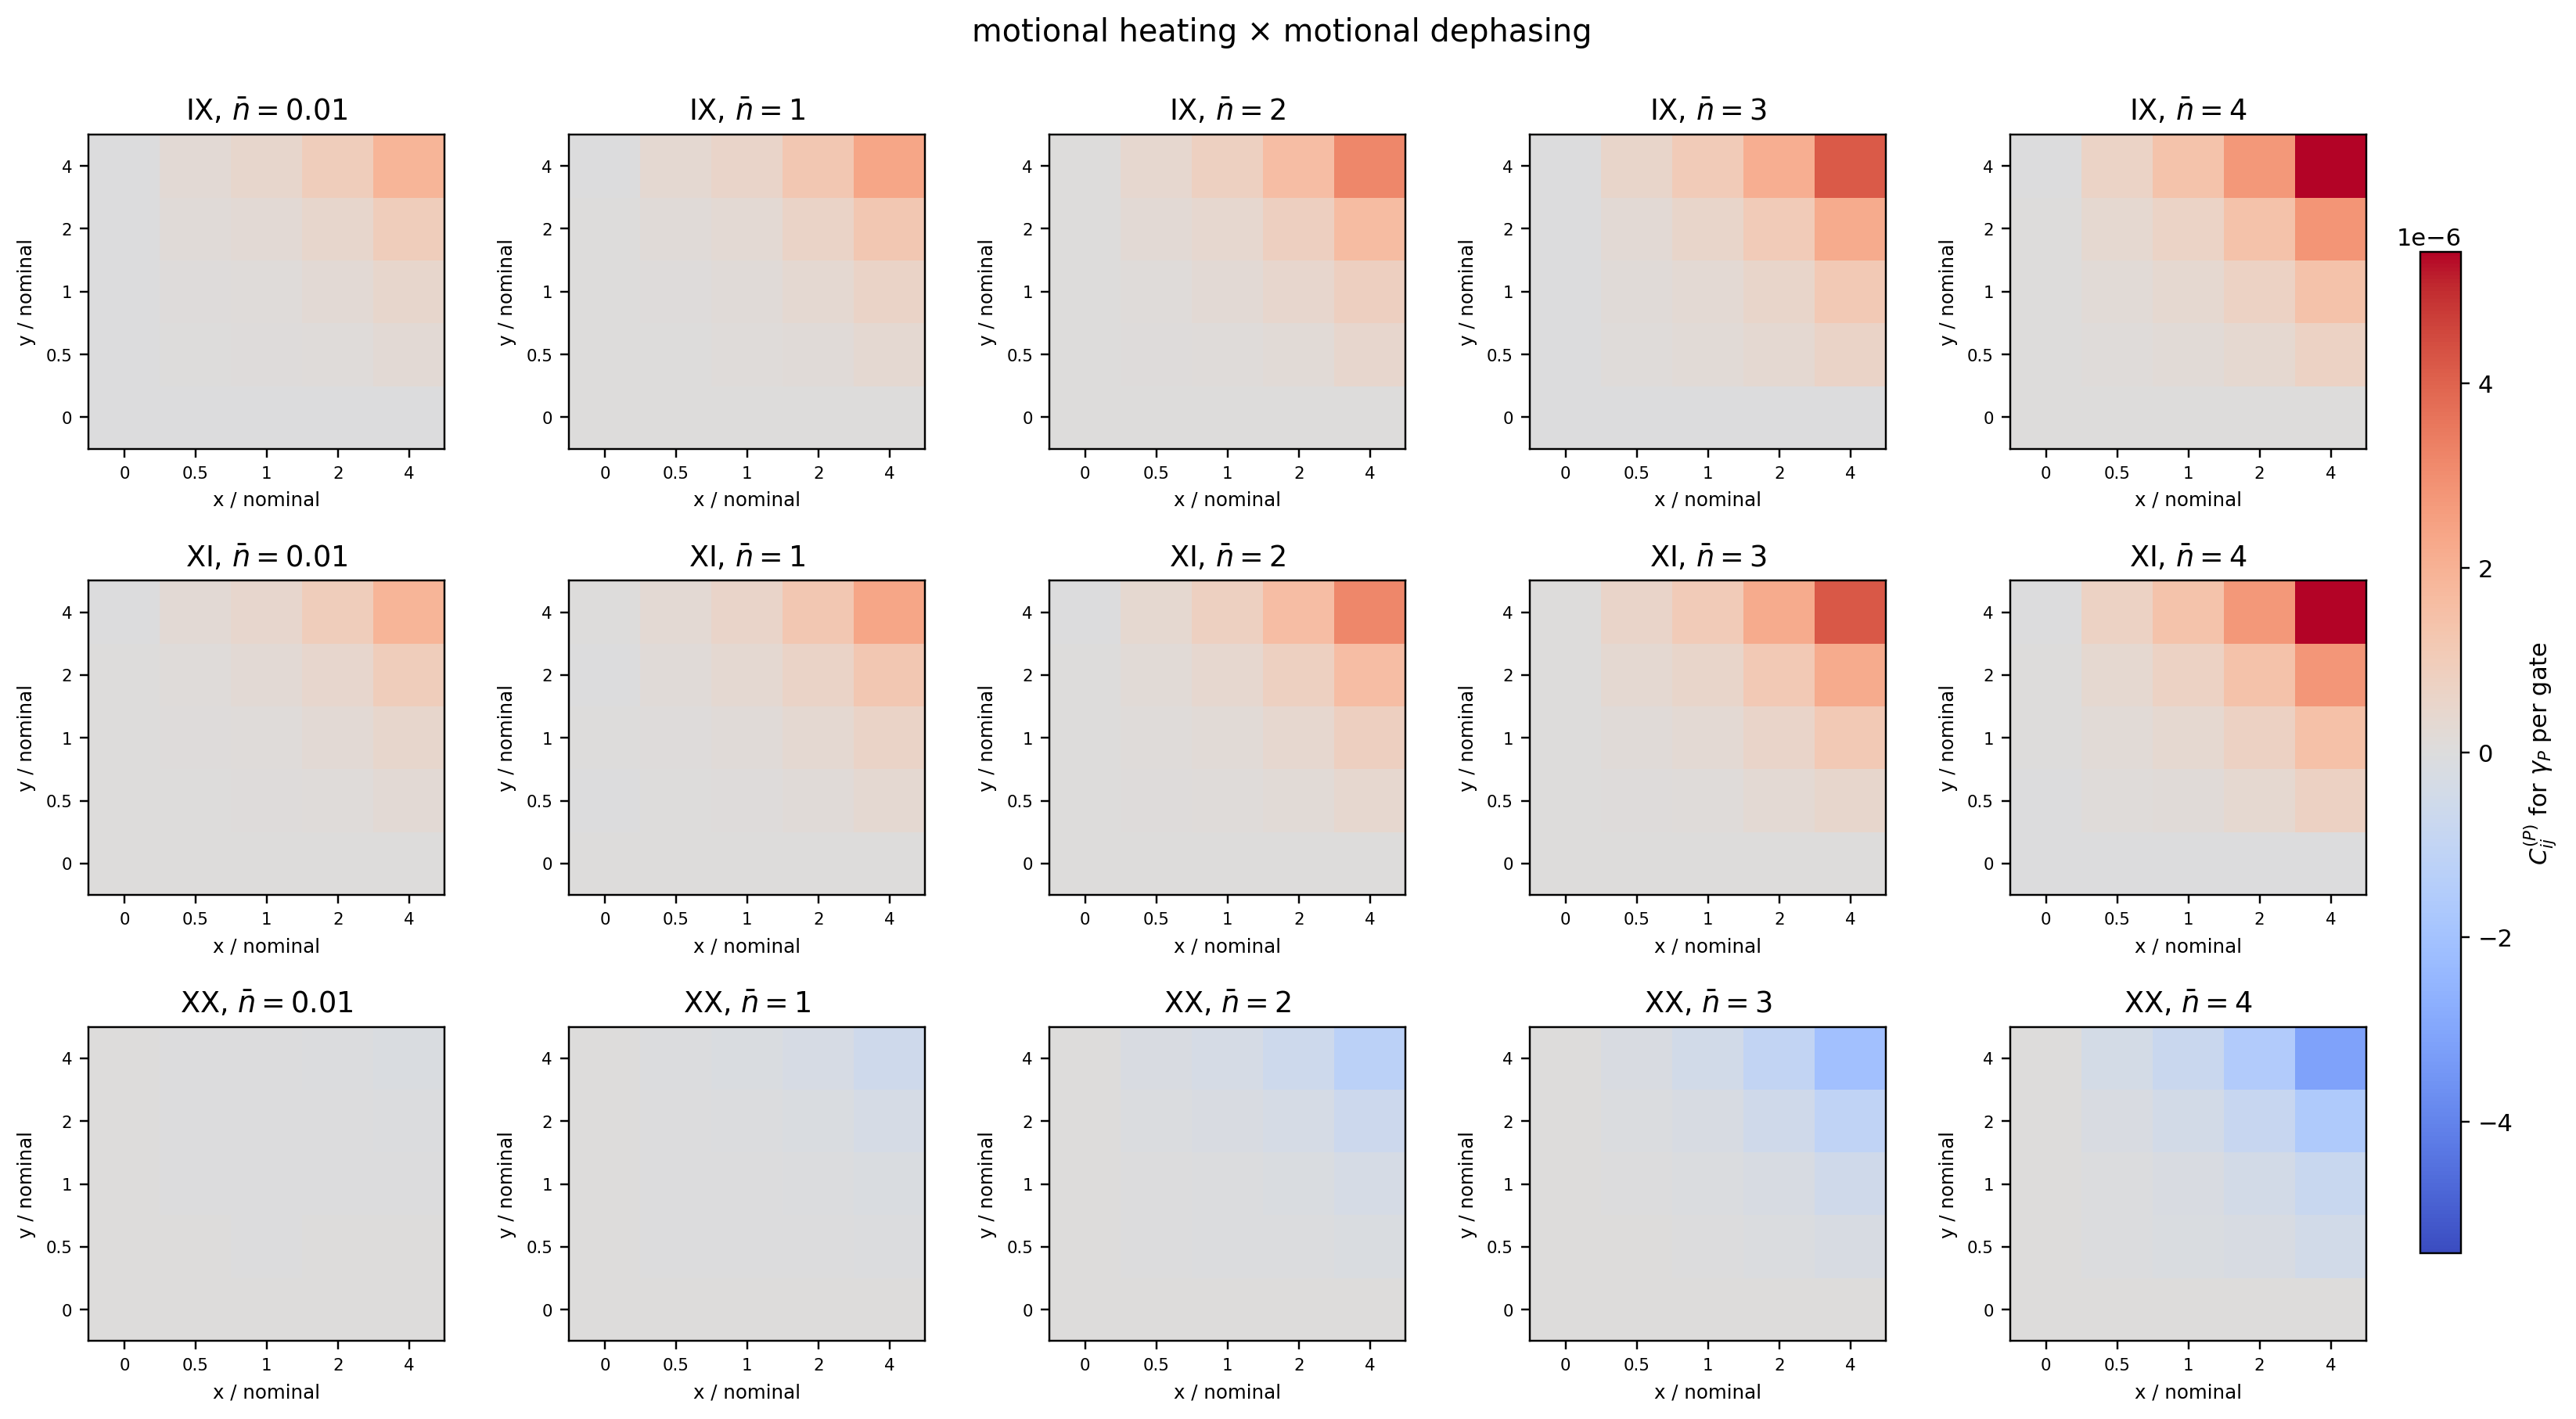
\includegraphics[width=0.96\textwidth]
{top_pauli_interactions__motional_heating__motional_dephasing.png}
\caption{Heatingとmotional dephasingに対する主要な
generator interaction．$IX/XI$は正，$XX$は負であり，
いずれも$\bar n$およびノイズ倍率とともに絶対値が増加する．}
\label{fig:interaction_maps}
\end{figure*}

\subsection{ノイズ倍率依存}

固定した$\bar n$では，主要成分はほぼ
\begin{align}
 C_{hd}^{(\gamma,IX/XI)}
 &\simeq +a_X(\bar n)m_hm_d,\\
 C_{hd}^{(\gamma,XX)}
 &\simeq -a_{XX}(\bar n)m_hm_d,\\
 C_{hd}^{(h,XX)}
 &\simeq +b_{XX}(\bar n)m_hm_d
\end{align}
に従った．$IX/XI$については各$\bar n$で
$R^2>0.998$である．

片方のノイズ倍率を固定するとinteractionはもう一方の倍率に
ほぼ線形に増加する．両方を同じ倍率$m$にすると
$m_hm_d=m^2$であるため，interactionはほぼ$m^2$に比例する．
したがって，両ノイズを半分にすると，その組合せ効果は
およそ$1/4$になる．調べた$m=0.5$--$4$の範囲では，
明確な閾値や飽和は確認されなかった．

また，$\bar n$の増加に伴い，$IX/XI$散逸の積係数は約3倍，
負の$XX$散逸の積係数は約23倍に増加した．一方，
$h_{XX}$の積係数は約半分に減少した．すなわち，低温では
コヒーレントなMS回転角補正が比較的重要であるが，高温では
散逸的なlocal $X$誤差と$XX$誤差の再配分が支配的になる．

\subsection{物理的解釈と限界}

単一ノイズ軸から構成したPauli-mode overlapでは，$IX/XI$が
overlap scoreの99.98\%を占め，direct pairwise QPTでも
$IX/XI$が最大の散逸interactionとなった．したがって，
heatingとmotional dephasingが共通してsingle-ion $X$型誤差を
強めるという解釈は支持される．

一方，direct QPTでは約22\%の$XX$散逸interactionと，
低温側で顕著な$h_{XX}$も確認された．したがって，
infidelityの非加法性をlocal散逸だけで説明することはできず，
\begin{enumerate}
 \item 同じ$IX/XI$散逸方向への作用，
 \item $XX$散逸の加算予想からの減少，
 \item coherentなMS回転角補正
\end{enumerate}
の組合せとして理解する必要がある．

motional dephasing $\times$ photon scatteringおよび
motional dephasing $\times$ spin dephasingの最大
$\gamma$ interactionは，heating $\times$ motional dephasing
より約6--10倍小さかった．このため，後者を主要な物理モデルとして
扱うことは妥当である．

なお，本解析の$C_{hd}^{(q,P)}$はerror channel上の
\textbf{dynamical nonadditivity}であり，heating浴とdephasing浴の
統計的相関を直接証明するものではない．浴相関を主張するには，
非対角Kossakowski成分または相互相関スペクトルを含むMEと，
独立浴モデルを比較する必要がある\cite{GKSL}．

また，Pauli-diagonal dissipator近似で説明されないgenerator成分が
中央値で約4.3\%，95 percentileで約14\%残る．したがって，
$10^{-8}$程度の小さいinteractionには物理的解釈を与えず，
滑らかな倍率依存とイオン交換対称性を示す$IX/XI$，$XX$成分に
議論を限定するのが安全である．

\section{Conclusion}

Heatingとmotional dephasingの同時作用は，熱占有数とともに
増加するgenerator-levelの非加法性を生む．その主成分は
single-ionの$IX/XI$散逸増強であるが，これを部分的に打ち消す
負の$XX$散逸interactionと，低温側で顕著なcoherent
$h_{XX}$補正も存在する．

実験的には，$h_{XX}$はパルス面積やdetuningの再較正により
補償できる可能性がある．一方，$\gamma_{IX/XI}$および
$\gamma_{XX}$はユニタリ補正では除去できないため，冷却，
heating抑制，運動コヒーレンス改善を同時に行う必要がある．

\begin{thebibliography}{99}
\small

\bibitem{MS}
A. S{\o}rensen and K. M{\o}lmer,
Phys. Rev. A \textbf{62}, 022311 (2000).

\bibitem{QPT}
I. L. Chuang and M. A. Nielsen,
J. Mod. Opt. \textbf{44}, 2455--2467 (1997).

\bibitem{GST}
E. Nielsen \textit{et al.},
Quantum \textbf{5}, 557 (2021).

\bibitem{Markovian_Errors}
Robin Blume-Kohout, Marcus P. da Silva, Erik Nielsen,
Timothy Proctor, Kenneth Rudinger, Mohan Sarovar, and
Kevin Young, “A Taxonomy of Small Markovian Errors”
arXiv:2103.01928.

\bibitem{GKSL}
G. Lindblad,
Commun. Math. Phys. \textbf{48}, 119--130 (1976);
V. Gorini, A. Kossakowski, and E. C. G. Sudarshan,
J. Math. Phys. \textbf{17}, 821--825 (1976).

\end{thebibliography}

\end{document}